\documentclass[letterpaper,11pt]{article}
\oddsidemargin -1.0cm \textwidth 17.5cm

\usepackage[utf8]{inputenc}
\usepackage[activeacute,spanish, es-lcroman]{babel}
\decimalpoint
\usepackage{amsfonts,setspace}
\usepackage{amsmath}
\usepackage{amssymb, amsmath, amsthm}
\usepackage{comment}
\usepackage{float}
\usepackage{amssymb}
\usepackage{dsfont}
\usepackage{anysize}
\usepackage{multicol}
\usepackage{enumerate}
\usepackage{graphicx}
\usepackage[left=1.5cm,top=2cm,right=1.5cm, bottom=1.7cm]{geometry}
\setlength\headheight{1.5em} 
\usepackage{fancyhdr}
\usepackage{multicol}
\usepackage{hyperref}
\usepackage{wrapfig}
\usepackage{subcaption}
\usepackage{siunitx}
\usepackage{cancel}
\usepackage{mdwlist}
\usepackage{svg}
\pagestyle{fancy}
\fancyhf{}
\renewcommand{\labelenumi}{\normalsize\bfseries P\arabic{enumi}.}
\renewcommand{\labelenumii}{\normalsize\bfseries (\alph{enumii})}
\renewcommand{\labelenumiii}{\normalsize\bfseries \roman{enumiii})}


\begin{document}

\fancyhead[L]{\itshape{Facultad de Ciencias F\'isicas y Matem\'aticas}}
\fancyhead[R]{\itshape{Universidad de Chile}}

\begin{minipage}{11.5cm}
    \begin{flushleft}
        \hspace*{-0.6cm}\textbf{FI1000-1 Introducción a la Física Clásica}\\
        \hspace*{-0.6cm}\textbf{Profesora:} Jocelyn Dunstan\\
        \hspace*{-0.6cm}\textbf{Auxiliar:} Alejandro Silva\\
        \hspace*{-0.6cm}\textbf{Ayudantes:} Macarena Muñoz \& Catalina Vargas\\
    \end{flushleft}
\end{minipage}

\begin{picture}(2,3)
    \svgpath{../}  % descomentar si se agrega a carpeta "auxiliares"/"ejercicios"
    \put(366, 10){\includesvg[scale=0.31]{img/dfi.svg}}
\end{picture}

\begin{center}
	\LARGE\textbf{Auxiliar \#7}\\
	\Large{Trabajo y Energía}
\end{center}

\vspace{-1cm}
\begin{enumerate}\setlength{\itemsep}{0.4cm}

\rfoot[]{pág. \thepage}

\item[]

\item Un bloque de masa $M$ comienza a deslizar, desde una altura $H$, por una cuña de ángulo característico $\alpha$. Si el coeficiente de roce es $\mu_c$, determine el trabajo realizado por la fuerza de roce y el peso.

\begin{figure}[H]
    \centering
    \svgpath{../img/aux7}
    \includesvg[width=0.25\linewidth]{p1.svg}
\end{figure}

\item En un parque de entretenciones un carro de masa $m$ se desliza por una rampla desde un altura $h$ ingresando a un loop de radio $R$. Para abaratar costos la altura $h$ desde donde se suelta el carro es la mínima para que el carro no se suelte de la vía. Emergiendo del loop el carro entra a una zona de frenado de largo $L$ que consiste en una plano con coeficiente de roce $\mu_c$. Sin embargo el carro no alcanza a frenar en la primera pasada, sino que pasa de largo y entra en contacto con un resorte de constante elástica $k$. Vuelve y reingresa a la zona de frenado donde se detiene justo en la mitad de este. Determine:

\begin{enumerate}
    \item La velocidad en el punto $B$
    \item La altura $h$
    \item El largo $L$
    \item La máxima compresión del resorte
\end{enumerate}

\begin{figure}[h!]
    \centering
    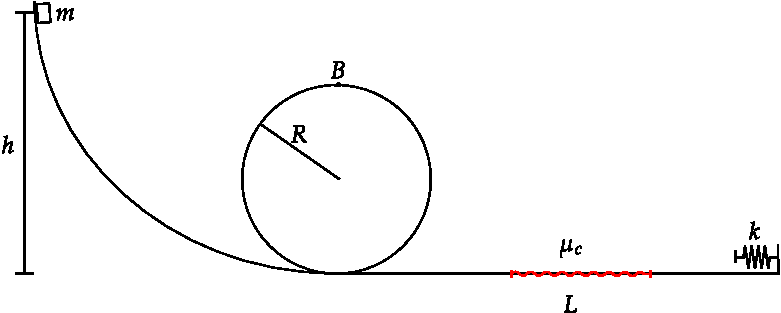
\includegraphics[scale=0.60]{2020-1/Imágenes/aux10/raptor.pdf}
\end{figure}

\item Considere una superficie horizontal rugosa que empalma suavemente con un tubo semicircular pulido de radio $R$. Un cubo pequeño de masa no nula es lanzado desde $P$ sobre la superficie, ingresa por el tubo y emerge desde su extremo superior hasta caer sobre el punto de partida $P$. La longitud del tramo rugoso es $D$ y el coeficiente de roce cinético con el cubo es $\mu$.
    \begin{enumerate}
        \item Determine la rapidez con la cual debe partir el cubo para que lo descrito sea posible.
        \item Analice e interprete su resultado para el caso $D \sim 0$
    \end{enumerate}

    \begin{figure}[H]
        \centering
        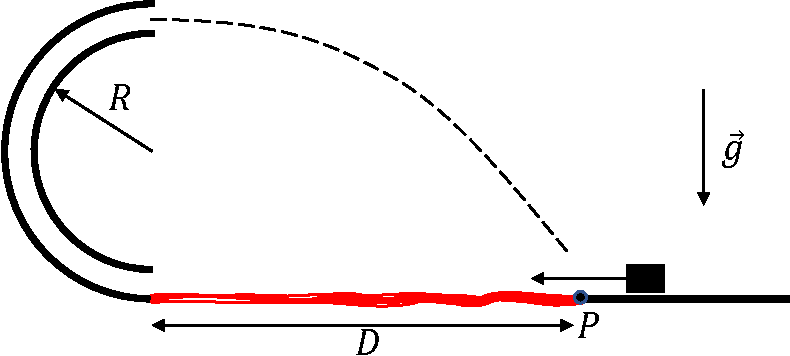
\includegraphics[scale=0.45]{2020-1/Imágenes/aux Extra-C2/p1_extra.pdf}
    \end{figure}


% Para imágenes vectoriales -> el texto tiene que estar en LaTeX
% \begin{figure}[htbp]
%   \centering
%   \svgpath{../Imagenes/ejercicios}  -> .. irse pa'trás 
%   \includesvg{ej5.svg}
% \end{figure}

\end{enumerate}
\end{document}
